\chapter{绪论}
绪论部分。。。。
\section{课题背景}
粘贴内容到此处

分段时空一行

粘贴内容到此处

%悬挂缩进
\noindent
\hangafter 1
\hangindent 2em
(1) 图像的获取:在进行相应的图像处理之前,先要用摄像机拍摄获取三维物体的二维图像,其中光照条件、相机的几何特性等会对之后的图像处理造成很大的影响。

%图片
\begin{figure}[!htbp]
	\centering
	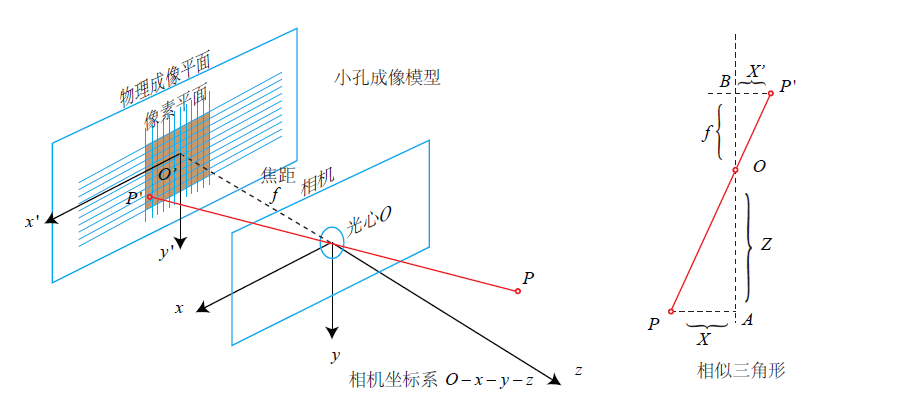
\includegraphics[width=1.00\textwidth]{myfigures/slam-01.png} %1.png是图片文件的相对路径
	\caption{东北大学东门建筑稀疏点云模型} %caption是图片的标题
	\label{neuxishu} %此处的label相当于一个图片的专属标志,目的是方便上下文的引用
\end{figure}

%算法
\begin{algorithm}
	\setstretch{1.25}
	\caption{DELAUNAYTRIANGULATION(P)}
	\begin{algorithmic}[1] %每行显示行号
		\Require 由平面上$n+1$个点组成一个集合$P$ 
		\Ensure $P$的一个Delaunay三角剖分
		\State 令$p_0$为$P$中依字典序最高的点,即纵坐标最大的点
		\State 在$R^2$中选取距离足够远的点$p_1$和$p_2$,将$P$完全包含于三角形$p_0p_1p_2$中
		\State 将$T$初始化为一个单独的三角形$p_0p_1p_2$
		\State 随机排列$P\setminus\{p_0\}$中的点 
		
		\For {$r \leftarrow 1$ \, $to$ \, $ n$: }
		\State (将$p_r$插入到$T$中)
		找到$p_r$所在的三角形$p_ip_jp_k \in T$ 
		\If{ $p_r$落在三角形$p_ip_jp_k$内部}
		\State 分别将$p_r$与三角形$p_ip_jp_k$的三个顶点相连(生成三条边) 
		\State	$LEGALIZEEDGE(p_r, \overline{p_ip_j}, T)$
		\State	$LEGALIZEEDGE(p_r, \overline{p_kp_j}, T)$ 
		\State	$LEGALIZEEDGE(p_r, \overline{p_kp_i}, T)$ 
		\ElsIf {$p_r$刚好落在三角形$p_ip_jp_k$的某一条边上(不妨设为$\overline{p_ip_j}$)}
		\State 将$p_r$分别与$p_k$以及与$\overline{p_ip_j}$关联的另一个三角形的第三个顶点$p_l$相连 
		\State (从而将与$\overline{p_ip_j}$相关联的那两个三角形划分为四个三角形) 
		\State $LEGALIZEEDGE(p_r, \overline{p_ip_l}, T)$ 
		\State $LEGALIZEEDGE(p_r, \overline{p_lp_j}, T)$ 
		\State $LEGALIZEEDGE(p_r, \overline{p_kp_j}, T)$ 
		\State $LEGALIZEEDGE(p_r, \overline{p_kp_i}, T)$ 
		\State $LEGALIZEEDGE(p_r, \overline{p_kp_i}, T)$ 
		\EndIf
		\EndFor
		\State 将点$p_1,p_2$以及与之关联的所有边从$T$中剔除掉 
		\State \Return{$T$}
	\end{algorithmic}
\end{algorithm}

%表格  https://blog.csdn.net/JueChenYi/article/details/77116011
\begin{table}[!htbp] 
	\centering
	\begin{tabular}{|c|c|c|}
		\hline
		\multicolumn{3}{|c|}{学生信息}\\ % 用\multicolumn{3}表示横向合并三列 
		% |c|表示居中并且单元格两侧添加竖线 最后是文本
		\hline
		姓名&学号&性别\\
		\hline
		Jack& 001& Male\\
		\hline
		Angela& 002& Female\\
		\hline
	\end{tabular}
	\caption{这是一张三线表}
\end{table}

\section{研究现状}
粘贴内容到此处\cite{7956190}

分段时空一行

粘贴内容到此处

